% !TEX root = report.tex

\subsubsection{\texttt{FORCLJ} subroutine}
\label{sssec:forclj}

The subroutine will first calculate the Cartesian distance between 2 atoms.
It will call \texttt{ELJ} subroutine for each pair of atoms $i$ and $j$, in which
the force between these $2$ atoms in both Cartesian and reduced coordinates
are calculated, and denoted as \texttt{fo} and \texttt{fos}, respectively.
More detailedly, \texttt{ELJ} uses the Lennard--Jones scheme.

The Lennard--Jones potential has general form
\begin{equation}
	U(r) = 4\varepsilon \bigg( \Big( \frac{ \sigma }{ r } \Big) ^ {12} -
	\Big( \frac{ \sigma }{ r } \Big) ^ 6 \bigg),
\end{equation}
where $r$ is the distance between $2$ atoms, $\sigma$ and $\varepsilon$
are constants.
The force is calculated by
\begin{equation}
	\bm{F}_{ji} = \frac{ 24\varepsilon }{ \sigma } (\bm{r}_j - \bm{r}_i)
	\bigg( 2\Big( \frac{ \sigma }{ r } \Big) ^ {14} -
	\Big( \frac{ \sigma }{ r } \Big) ^ 8 \bigg),
\end{equation}
where $r = \lvert \bm{r}_j - \bm{r}_i \rvert$, or equivalently, its scalar form
\begin{equation}
	F(r) = \frac{ 24\varepsilon }{ \sigma }
	\bigg( 2\Big( \frac{ \sigma }{ r } \Big) ^ {13} -
	\Big( \frac{ \sigma }{ r } \Big) ^ 7 \bigg),
\end{equation}
which is plotted in Fig. \ref{fig:ljar}.

\begin{figure}[h]
	\centering
	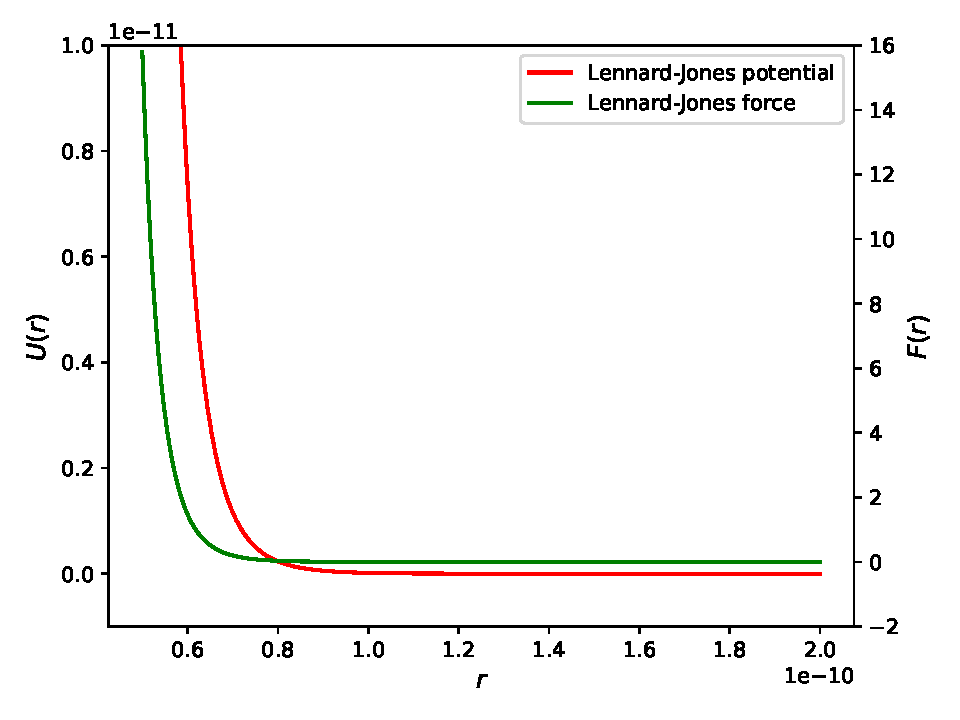
\includegraphics[width=0.5\linewidth]{lj_ar.pdf}
	\caption{Lennard--Jones potential and force for $\ce{Ar}$, as a function of
		distance between $2$ atoms, with
		$\sigma=3.405\times 10^{-10}\si{\meter}$,
		$\varepsilon = 1.654\times 10^{-21}\si{\joule}$.\cite{buffalomd}}
	\label{fig:ljar}
\end{figure}

Back to \texttt{FORCLJ} subroutine,
it considers 2 cases: particle $j$ and $i$ in the same cell and
in different cells, the first case is trivial, in the second case,
we need to add multiple times of primitive vectors and then calculate distance
$r_{ji}$, and the rest steps are the same as first case. In both cases, we do not
consider interaction out of the radius $r_{\text{cut}}$.
It appends \texttt{fo} and \texttt{fos} modified by \texttt{ELJ}
subroutine to the \texttt{f} and \texttt{fs}, respectively.
